% Homework template for Information Theory and Statistical Learning
% by Xiangxiang Xu <xiangxiangxu.thu@gmail.com>
% LAST UPDATE: Oct 3, 2019
\documentclass[a4paper]{article}
\usepackage[T1]{fontenc}
\usepackage{amsmath, amssymb, amsthm}
% amsmath: equation*, amssymb: mathbb, amsthm: proof
\usepackage{moreenum}
\usepackage{mathtools}
\usepackage{url}
\usepackage{enumitem}
\usepackage{bm}
\usepackage{graphicx}
\usepackage{hyperref}
\usepackage{subcaption}
\usepackage{booktabs} % toprule
\usepackage[mathcal]{eucal}
\usepackage{dsfont}
\usepackage[numbered,framed]{matlab-prettifier}
%% Definitions for Information Theory & Statistical Learning
%% UPDATED: Sep 30, 2019 by Xiangxiang 
\newcommand{\theterm}{Fall 2020}

\newcommand{\thecoursenameshort}{\textsc{Information Theory and Statistical Learning}}
\newcommand{\thecoursename}{
Tsinghua-Berkeley Shenzhen Institute\\
%\vspace*{0.1in}
\thecoursenameshort
}

\newcommand{\courseheader}{
\vspace*{-1in}
\begin{center}
\thecoursename \\
\theterm
\vspace*{0.1in}
\hrule
\end{center}
}
\newcommand{\uc}{\underline{c}}    % c, vec
\newcommand{\uv}{\underline{v}}    % x, vec
\newcommand{\uw}{\underline{w}}    % w, vec
\newcommand{\ux}{\underline{x}}    % x, vec
\newcommand{\uy}{\underline{y}}    % y, vec
\newcommand{\uz}{\underline{z}}    % z, vec
\newcommand{\um}{\underline{m}}    % m, vec
\newcommand{\ut}{\underline{t}}    % t, vec

\newcommand{\bA}{\mathbf{A}}    % A, mat
\newcommand{\bI}{\mathbf{I}}    % A, mat
\newcommand{\bN}{\mathbf{N}}    % n, mat
\newcommand{\bT}{\mathbf{T}}    % T, mat
\newcommand{\bU}{\mathbf{U}}    % U, mat
\newcommand{\bV}{\mathbf{V}}    % V, mat
\newcommand{\bQ}{\mathbf{Q}}    % Q, mat
\newcommand{\bX}{\mathbf{X}}    % X, mat

\newcommand{\bc}{\bm{c}}    % c, vec
\newcommand{\be}{\bm{e}}    % e, vec
\newcommand{\bu}{\bm{u}}    % u, vec
\newcommand{\bv}{\bm{v}}    % v, vec
\newcommand{\bw}{\bm{w}}    % w, vec
\newcommand{\bt}{\bm{t}}    % t, vec
\newcommand{\bx}{\bm{x}}    % x, vec
\newcommand{\by}{\bm{y}}    % y, vec
\newcommand{\bz}{\bm{z}}    % z, vec

\newcommand{\phib}{\bm{\phi}}    % phi, vec
\newcommand{\psib}{\bm{\psi}}    % psi, vec
\newcommand{\dtm}{\mathbf{B}}    %
\newcommand{\dtmt}{\tilde{\dtm}}    %
\newcommand{\Ab}{\mathbf{A}}    % A mat
\newcommand{\Kb}{\mathbf{K}}    % K mat
\newcommand{\Ib}{\mathbf{I}}    % I mat



\newcommand{\rvby}{\bm{\mathsf{y}}}    % y, rv. vec
\newcommand{\rvbx}{\bm{\mathsf{x}}}    % x, rv. vec
% \newcommand{\bm}{\bm{m}}    % m, vec
\newcommand{\bzero}{\bm{0}}    % 0, vec

\newcommand{\balpha}{\bm{\alpha}}    % alpha, vec
\newcommand{\bphi}{\bm{\phi}}    % phi, vec
\newcommand{\bpsi}{\bm{\psi}}    % psi, vec
\newcommand{\bxi}{\bm{\xi}}    % xi, vec
\newcommand{\btheta}{\bm{\theta}}    % theta, vec
\newcommand{\bmu}{\bm{\mu}}    % mu, vec

\newcommand{\bLambda}{\bm{\Lambda}}    % Sigma, mat
\newcommand{\bSigma}{\bm{\Sigma}}    % Sigma, mat

\newcommand{\cF}{\mathcal{F}}  
\newcommand{\cL}{\mathcal{L}}  
\newcommand{\cX}{\mathcal{X}}  
\newcommand{\cY}{\mathcal{Y}}  

\newcommand{\rvx}{\mathsf{x}}    % x, r.v.
\newcommand{\rvy}{\mathsf{y}}    % y, r.v.
\newcommand{\rvz}{\mathsf{z}}    % z, r.v.
\newcommand{\rvw}{\mathsf{w}}    % w, r.v.
\newcommand{\rvv}{\mathsf{v}}    % v, r.v.
\newcommand{\rvm}{\mathsf{m}}    % m, r.v.
\newcommand{\rvt}{\mathsf{t}}    % t, r.v.
\newcommand{\rvH}{\mathsf{H}}    % H, r.v.
\newcommand{\urvx}{\underline{\mathsf{x}}}    % x, r.v. vec
\newcommand{\urvy}{\underline{\mathsf{y}}}    % y, r.v. vec
\newcommand{\urvz}{\underline{\mathsf{z}}}    % z, r.v. vec
\newcommand{\urvw}{\underline{\mathsf{w}}}    % w, r.v. vec
\newcommand{\urvt}{\underline{\mathsf{t}}}    % t, r.v. vec


\newcommand{\defeq}{\triangleq} %\coloneqq
\newcommand{\reals}{\mathbb{R}}
\newcommand{\T}{\mathrm{T}}    % transpose
\newcommand{\F}{\mathrm{F}}    % Frobenius
\newcommand{\BLS}{\mathrm{BLS}}    % BLS
\newcommand{\LLS}{\mathrm{LLS}}    % LLS
\newcommand{\MVU}{\mathrm{MVU}}    % MVU
\newcommand{\dd}{\mathrm{d}}  

\DeclareMathOperator*{\maximize}{maximize}    % maximize
\DeclareMathOperator*{\minimize}{minimize}    % minimize
\newcommand{\st}{\mathrm{subject~to}}    % minimize

% \newcommand{\E}[1]{\mathbb{E}\left[{#1}\right]}
% \newcommand{\Prob}[1]{\mathbb{P}\left({#1}\right)}
\DeclareMathOperator*{\argmax}{arg\,max}
\DeclareMathOperator*{\argmin}{arg\,min}
\DeclareMathOperator*{\argsup}{arg\,sup}
\DeclareMathOperator*{\arginf}{arg\,inf}
\DeclareMathOperator{\diag}{diag}
\DeclareMathOperator{\tr}{tr}
\DeclareMathOperator{\Cov}{Cov}
\DeclareMathOperator{\var}{var}
\DeclareMathOperator{\cov}{cov}
\DeclareMathOperator{\MSE}{MSE}
\DeclareMathOperator{\1}{\mathds{1}} % dsfont required
\DeclareMathOperator{\E}{\mathbb{E}}
\DeclareMathOperator{\Prob}{\mathbb{P}}
\DeclareMathOperator{\im}{im}
\DeclareMathOperator{\rank}{rank}
\DeclareMathOperator{\Bern}{Bern}
\DeclareMathOperator{\Binom}{Binom}

\newcommand\independent{\protect\mathpalette{\protect\independenT}{\perp}}
\def\independenT#1#2{\mathrel{\rlap{$#1#2$}\mkern2mu{#1#2}}}

%%% Local Variables:
%%% mode: latex
%%% TeX-master: "ithw"
%%% End:


\lstset{
  style              = Matlab-editor,
  captionpos         =b,
  basicstyle         = \mlttfamily,
  escapechar         = ",
  mlshowsectionrules = true,
}
\begin{document}
\courseheader



\newcounter{hwcnt}
\setcounter{hwcnt}{3} % set to the times of Homework

\begin{center}
  \underline{\bf Homework \thehwcnt} \\
\end{center}
\begin{flushleft}
  \textcolor{gray}{YOUR NAME}\hfill
  \today
\end{flushleft}
\hrule

\vspace{2em}
\setlist[enumerate,1]{label=\thehwcnt.\arabic*.}
\setlist[enumerate,2]{label=(\alph*)}
\setlist[enumerate,3]{label=\roman*.}
\setlist[enumerate,4]{label=\greek*)}

\flushleft
\rule{\textwidth}{1pt}
\begin{itemize}
\item {\bf Acknowledgments: \/} 
  \textcolor{gray}{For Problem 3.3(b), I refer to the lecture notes of  Madhur Tulsiani, University of Chicago \url{https://ttic.uchicago.edu/~madhurt/courses/infotheory2014/l5.pdf}. For Problem 3.6(b)-(d), I refer to the essay \textbf{Detection with Distributed Sensors} by Robert R. Tenney \url{https://ieeexplore.ieee.org/abstract/document/4102537}}

\item {\bf Collaborators: \/}
  \textcolor{gray}{I finish this template by myself.} 

\item  \emph{I certify that all solutions are entirely in my words and that I have not looked at another student's solutions. I have credited all external sources in this write up.}
  \framebox[\linewidth]{\rule{0pt}{10pt}\textcolor{gray}{\large Hanmo Chen}}
\end{itemize}
\rule{\textwidth}{1pt}


\vspace{2em}



\begin{enumerate}
  \setlength{\itemsep}{3\parskip}

\item \begin{enumerate}% 3.1
  \item First we have,
  \begin{equation}
    \begin{aligned}
      \sum_{x \in \mathcal{X}} P_{\mathrm{y}}(x) D\left(P_{\mathrm{y} \mid \mathrm{x}=x} \| P_{\mathrm{y} \mid \mathrm{x}=x_{0}}\right) & = \sum_{x \in \mathcal{X}}   P_{\mathrm{y}}(x) \left(\sum_{y\in \mathcal{Y}} P_{\mathrm{y}|\mathrm{x}=x}(y) \log \frac{P_{\mathrm{y}|\mathrm{x}=x}(y)}{P_{\mathrm{y}|\mathrm{x}=x_0}(y)}\right) \\
      & = \sum_{x \in \mathcal{X}}   P_{\mathrm{x}}(x) \left(\sum_{y\in \mathcal{Y}} P_{\mathrm{y}|\mathrm{x}=x}(y) \log \frac{P_{\mathrm{x},\mathrm{y}}(x,y)}{P_{\mathrm{x}}(x)P_{\mathrm{y}|\mathrm{x}=x_0}(y)}\right) \\
      & = \sum_{x \in \mathcal{X}}   P_{\mathrm{x}}(x) \left[\sum_{y\in \mathcal{Y}} P_{\mathrm{y}|\mathrm{x}=x}(y) \left(\log \frac{P_{\mathrm{x},\mathrm{y}}(x,y)}{P_{\mathrm{x}}(x)P_{\mathrm{y}}(y)} + \log \frac{P_{\mathrm{y}}(y)}{P_{\mathrm{y}|\mathrm{x}=x_0}(y)}\right )\right] \\
      & = \sum_{x,y \in \mathcal{X} \times \mathcal{Y}} P_{\mathrm{x}}(x) P_{\mathrm{y}|\mathrm{x}=x}(y) \log \frac{P_{\mathrm{x},\mathrm{y}}(x,y)}{P_{\mathrm{x}}(x)P_{\mathrm{y}}(y)} \\
      &\quad +  \sum_{x,y \in \mathcal{X} \times \mathcal{Y}} P_{\mathrm{x}}(x) P_{\mathrm{y}|\mathrm{x}=x}(y) \log \frac{P_{\mathrm{y}}(y)}{P_{\mathrm{y}|\mathrm{x}=x_0}(y)}
    \end{aligned}
  \end{equation}


And because $P_{\mathrm{x}}(x)P_{\mathrm{y}|\mathrm{x}=x}(y) = P_{\mathrm{x},\mathrm{y}}(x,y)$ and $\log \frac{P_{\mathrm{y}}(y)}{P_{\mathrm{x}|\mathrm{x}=x_0}(y)}$ is independent of $y$, we have,

\begin{equation}
  \begin{aligned}
    \sum_{x \in \mathcal{X}} P_{\mathrm{x}}(x) D\left(P_{\mathrm{y} \mid \mathrm{x}=x} \| P_{\mathrm{y} \mid \mathrm{x}=x_{0}}\right) & = I(X;Y) + \sum_{y\in \mathcal{Y}} P_{\mathrm{y}}(y)  \log \frac{P_{\mathrm{y}}(y)}{P_{\mathrm{y}|\mathrm{x}=x_0}(y)} \\
    & = I(X;Y) + D(P_{\mathrm{y}} || P_{\mathrm{y}|\mathrm{x}=x_0})
  \end{aligned}
\end{equation}

That is,

\begin{equation}
  I(X;Y) =   \sum_{x \in \mathcal{X}} P_{\mathrm{x}}(x) D\left(P_{\mathrm{y} \mid \mathrm{x}=x} \| P_{\mathrm{y} \mid \mathrm{x}=x_{0}}\right) -   D(P_\mathrm{y} || P_{\mathrm{y}|\mathrm{x}=x_0})
\end{equation}

\item 

From the last formula and $D(P_\mathrm{y} || P_{\mathrm{y}|\mathrm{x}=x_0}) \geqslant 0$ we know that $\forall x_0$,

\begin{equation}
  I(X;Y) \leqslant  \sum_{x \in \mathcal{X}} P_{\mathrm{x}}(x) D\left(P_{\mathrm{y} \mid \mathrm{x}=x} \| P_{\mathrm{y} \mid \mathrm{x}=x_{0}}\right) 
\end{equation}

And $\sum_{x \in \mathcal{X}} P_{\mathrm{x}}(x) = 1$, thus

\begin{equation}
  \sum_{x \in \mathcal{X}} P_{\mathrm{x}}(x) D\left(P_{\mathrm{y} \mid \mathrm{x}=x} \| P_{\mathrm{y} \mid \mathrm{x}=x_{0}}\right)  \leqslant \sup_{x\in \mathcal{X}} D\left(P_{\mathrm{y} \mid \mathrm{x}=x} \| P_{\mathrm{y} \mid \mathrm{x}=x_{0}}\right)  
\end{equation}

So 

\begin{equation}
  I(X;Y) \leqslant \sup_{x,x_0\in \mathcal{X}} D\left(P_{\mathrm{y} \mid \mathrm{x}=x} \| P_{\mathrm{y} \mid \mathrm{x}=x_{0}}\right)  
\end{equation}

\end{enumerate}

\item \begin{enumerate} % 3.2
  \item First we prove that $H(\mathrm{x};\mathrm{y};\mathrm{z}) \leqslant H(\mathrm{x};\mathrm{y}) + H(\mathrm{x};\mathrm{z}) - H(\mathrm{x})$,
  
  \begin{equation}
    \begin{aligned}
      H(\mathrm{x};\mathrm{y};\mathrm{z}) & = H(\mathrm{y};\mathrm{z} \mid \mathrm{x}) - H(\mathrm{x})\\ & \leqslant   H(\mathrm{y} \mid \mathrm{x})  + H(\mathrm{z} \mid \mathrm{x})- H(\mathrm{x}) = H(\mathrm{x};\mathrm{y}) + H(\mathrm{x};\mathrm{z})  - H(\mathrm{x})
    \end{aligned}
  \end{equation}

  Symmetrically, $H(\mathrm{x};\mathrm{y};\mathrm{z}) \leqslant H(\mathrm{x};\mathrm{y}) + H(\mathrm{y};\mathrm{z}) - H(\mathrm{y})$, thus

  \begin{equation}
    \begin{aligned}
      2 H(\mathrm{x};\mathrm{y};\mathrm{z}) & \leqslant 2H(\mathrm{x};\mathrm{y}) + H(\mathrm{x};\mathrm{z})+ H(\mathrm{y};\mathrm{z})- H(\mathrm{x})- H(\mathrm{y}) \\ & \leqslant H(\mathrm{x};\mathrm{y}) + H(\mathrm{x};\mathrm{z})+ H(\mathrm{y};\mathrm{z})
    \end{aligned}
  \end{equation}

  \item Place $n$ points in $\mathbb{R}^3$ arbitrarily. Let $(x,y,z)$ be the random variables uniformly distributed among those points, so $H(x,y,z) = \log (n)$. 
  
  \begin{equation}
    \begin{aligned}
      2 H(\mathrm{x};\mathrm{y};\mathrm{z}) &  \leqslant H(\mathrm{x};\mathrm{y}) + H(\mathrm{x};\mathrm{z})+ H(\mathrm{y};\mathrm{z}) \leqslant \log |\mathcal{X}\times \mathcal{Y}| + \log |\mathcal{Y}\times \mathcal{Z}| + \log |\mathcal{X}\times \mathcal{Z}|  = \log(n_1n_2n_3)
    \end{aligned}
  \end{equation}

  Thus 

  \begin{equation}
    n_1n_2n_3 \geqslant n^2
  \end{equation}
\end{enumerate}
  
\item \begin{enumerate} %3.3
  \item To simplify, we use the natural logarithm. denote $f(p,q) = p \ln \frac{p}{q} + (1-p)\ln \frac{1-p}{1-q} - 2(p-q)^2$.
  
  \begin{equation}
    \begin{aligned}
      \frac{\partial f}{\partial q} & = \frac {p}{q} - \frac {1-p}{1-q}-4(p-q) = \frac{p-q}{q(1-q)} -4 (p-q) \\
      & = (p-q)[\frac 1 {q(1-q)} - 4]
    \end{aligned}
  \end{equation}

  For fixed $p$, $\frac{\partial f}{\partial q} \leqslant 0$ when $q<p$ and $\frac{\partial f}{\partial q} \geqslant 0$ when $q>p$. So to minimize $f(p,q)$, $q_{\min}=p$ and $f(p,p)=0$, therefore  

  \begin{equation}
    p \ln \frac{p}{q} + (1-p)\ln \frac{1-p}{1-q}  \geqslant 2(p-q)^2
  \end{equation}

  \item Also use the natural logarithm. We need to prove 
  
  \begin{equation}\label{eq:pinsker}
    \operatorname{TV}(P, Q) \triangleq \sup _{E \in \mathcal{F}}(P(E)-Q(E))\leqslant \sqrt{{2} D(P \| Q)} 
  \end{equation}
  
  Consider the event $E^* = \{w| P(w)\geqslant Q(w)  \}$, so that $\operatorname{TV}(P, Q) \triangleq \sup _{E \in \mathcal{F}}(P(E)-Q(E)) = P(E^*) - Q(E^*)$

  And $P(E^*) + P(E^{*c}) = Q(E^*) + Q(E^{*c}) = 1$, so $|P(E^*) -Q(E^*)|= | P(E^{*c})- Q(E^{*c})|$,  which means,


  \begin{equation}\label{eq:tv}
    \begin{aligned}
      \operatorname{TV}(P, Q)&  = P(E^*) - Q(E^*) \\ 
      &= \frac 1 2 \left(|P(E^*) -Q(E^*)|+| P(E^{*c})- Q(E^{*c})|\right) \\
      & = \frac 1 2\sum_{w\in \Omega} |P(w)-Q(w)| = \frac 1 2 \|P-Q \|_1
    \end{aligned}
  \end{equation}

  Updating Equation \ref{eq:pinsker} with Equation \ref{eq:tv}, we just need to prove 

  \begin{equation}
    \frac 1 2 \|P-Q \|^2_1 \leqslant  D(P \| Q)
  \end{equation}
  
  Let $X$ be the indicator random variable of event $E^*$, that is

  \begin{equation}
    X(w) = \mathbf{I}(E^*) = \left\{ \begin{aligned}
      1, \text{ if } P(w) \geqslant Q(w) \\
      0, \text{ if } P(w) < Q(w)
    \end{aligned}
      \right.
  \end{equation}

  So $X$ is a bernoulli random variable with probability $P(E^*),Q(E^*)$, which we denote as the bernoulli distriburion $P_X,Q_X$ with probability $p,q$.

  Using the conclusion from (a), 

  \begin{equation}
    \begin{aligned}
      \frac 1 2 \|P-Q \|^2_1 = \frac{1}{2} (|p-q|+|(1-p)-(1-q)|^2 = 2(p-q)^2 \leqslant  D(P_X||Q_X)
    \end{aligned}
  \end{equation}
  

  And use the data processing inequality $D(P_X||Q_X) \leqslant D(P\| Q)$, so we prove that 

  \begin{equation}
    \operatorname{TV}(P, Q) \leqslant \sqrt{{2} D(P \| Q)} 
  \end{equation}

\end{enumerate}

\item \begin{enumerate} % 3.4
  \item Decision rule
  \begin{equation}
    \begin{aligned}
      \hat H(y) & = \argmax_{H_{i,i=0,1}} p_{\mathrm{H}| \mathrm{y}}(H_i|y) \\
      & = \argmax_{H_{i,i=0,1}} \frac {p_{\mathrm{y} | \mathrm{H}}(y| H_i)p(H_i)}{\sum_{i=0,1} p_{\mathrm{y} | \mathrm{H}}(y| H_i)p(H_i)} \\ 
      & = \argmax_{H_{i,i=0,1}} p_{\mathrm{y} | \mathrm{H}}(y| H_i)p(H_i)
    \end{aligned}
  \end{equation}

  \begin{itemize}
    \item For $H_0$, $p_{\mathrm{y} | \mathrm{H}}(y| H_0)p(H_0) = p,0\leqslant y \leqslant 1$
    \item For $H_1$, $p_{\mathrm{y} | \mathrm{H}}(y| H_1)p(H_1) = 2y(1-p),0\leqslant y \leqslant 1$
  \end{itemize}

  So  if $p <\frac {2}{3}$

  \begin{equation}
    \hat H(y) = \argmax_{H_{i,i=0,1}} p_{\mathrm{y} | \mathrm{H}}(y| H_i)p(H_i) = \left\{ \begin{aligned}
      H_0, \quad y \leqslant \frac{p}{2(1-p)} \\
      H_1, \quad y >  \frac{p}{2(1-p)}
    \end{aligned}\right.
  \end{equation}

  If $p\geqslant \frac {2}{3},  \hat H(y) = H_0$. 

  \item The Likelihood Ratio is,
  \begin{equation}
    \operatorname{LRT}(y) = \frac {p_{\mathrm{y} | \mathrm{H}}(y| H_0)}{p_{\mathrm{y} | \mathrm{H}}(y| H_1)} = \frac 1 {2y} \geqslant \lambda
  \end{equation}
  
  For $P_{\mathrm{D}}$, let $c = \frac {1}{2\lambda},\lambda \in [\frac 1 2,\infty)$

  \begin{equation}\label{eq:pd}
    \begin{aligned}
      P_{\mathrm{D}} \triangleq \mathbb{P}\left(\hat{\mathrm{H}}=H_{1} \mid \mathrm{H}=H_{1}\right) = \mathbb{P}(y> c | H = H_1) = 1-c^2
    \end{aligned}
  \end{equation}

  For $P_{\mathrm{F}}$,

  \begin{equation}
    \begin{aligned}
      P_{\mathrm{F}} \triangleq \mathbb{P}\left(\hat{\mathrm{H}}=H_{1} \mid \mathrm{H}=H_{0}\right) = \mathbb{P}(y> c | H = H_0) = 1-c
    \end{aligned}
  \end{equation}

  Replace $c$ with $1-P_{\mathrm{F}}$ in equation \ref{eq:pd}, we find the operating characteristic of LRT as

  \begin{equation}\label{eq:oc}
    P_{\mathrm{D}} = (2-P_{\mathrm{F}}) P_{\mathrm{F}}
  \end{equation}

  \item \begin{enumerate}
    \item Because $ P_{\mathrm{D}} = (2-P_{\mathrm{F}}) P_{\mathrm{F}}$, let $P_D \geqslant (1+\epsilon) P_{\mathrm{F}}$, we have  $P_{\mathrm{F}} \leqslant (1-\epsilon)$.  And  $P_{\mathrm{D}}$ is a monotonically increasing function of $P_{\mathrm{F}}$ in [0,1], so $P_{\mathrm{D}}^{\max}(\epsilon) = 1- \epsilon^2$ 
    \item $P_{\mathrm{D}}^{\max}(\epsilon) = 1- \epsilon^2 >0$ so $\epsilon \in (0,1)$ 
    \item In the decision rule from part (a), $P_{\mathrm{F}} = 1-\frac{p}{2(1-p)} \leqslant 1- \epsilon$, that is $p \geqslant \frac {2\epsilon}{1+2\epsilon}$
  \end{enumerate}
\end{enumerate}

\item \begin{enumerate} %3.5
  \item \begin{enumerate}
    \item The cost is 
  
    \begin{equation}
      \mathbb{E}[c(f(\underline{y}),H)] = \sum_{i=1}^3 P_{\underline{\mathrm{y}}}(\underline{y}) \mathbf{I}(f(\underline{y}) = H_i) \left( \sum_{j=1}^3 C_{ij}\pi_i(\underline{y}) \right)
    \end{equation}
  
    So
  
    \begin{equation}
      \hat H = f(\underline{y}) = \argmin_{i} \sum_{j=1}^3 C_{ij}\pi_i(\underline{y})
    \end{equation}
  
    Specifically,
  
    \begin{equation}
      \left\{
        \begin{aligned}
          l_1(\underline{y}) = \pi_{2}(\underline{y}) + 2 \pi_3({\underline{y}}) \\
          l_2(\underline{y}) = \pi_{1}(\underline{y}) + 2 \pi_3({\underline{y}}) \\
          l_3 (\underline{y})= 2\pi_{1}(\underline{y}) + 2 \pi_2({\underline{y}})
        \end{aligned}
      \right.
    \end{equation}
  
    \begin{enumerate}
      \item $ \hat H = H_1$: let $ l_1(\underline{y}) < l_2(\underline{y})$and  $ l_1(\underline{y}) <l_3 (\underline{y})$ we have $\pi_1(\underline{y}) > \pi_2(\underline{y})$ and $2\pi_3(\underline{y})<2\pi_1(\underline{y}) + \pi_2(\underline{y})$
      \item $ \hat H = H_2$: let $ l_2(\underline{y}) < l_1(\underline{y})$and  $ l_2(\underline{y}) <l_3 (\underline{y})$ we have $\pi_1(\underline{y}) < \pi_2(\underline{y})$ and $2\pi_3(\underline{y})<\pi_1(\underline{y}) + 2\pi_2(\underline{y})$
      \item $ \hat H = H_3$: let $ l_3(\underline{y}) < l_2(\underline{y})$and  $ l_3(\underline{y}) <l_1 (\underline{y})$ we have $2\pi_3(\underline{y})> 2\pi_1(\underline{y}) + \pi_2(\underline{y})$ and  $2\pi_3(\underline{y})> \pi_1(\underline{y}) + 2\pi_2(\underline{y})$
    \end{enumerate}
  
    So the optimum decision rule is,

    \begin{equation}
      \hat H = f(\underline{y}) = \left\{
        \begin{aligned}
          &H_1, \quad \pi_1(\underline{y}) > \pi_2(\underline{y}) \text{ and } 2\pi_3(\underline{y})<2\pi_1(\underline{y}) + \pi_2(\underline{y}) \\
          &H_2, \quad \pi_1(\underline{y}) < \pi_2(\underline{y}) \text{ and } 2\pi_3(\underline{y})<\pi_1(\underline{y}) + 2\pi_2(\underline{y}) \\
          &H_3, \quad 2\pi_3(\underline{y})> 2\pi_1(\underline{y}) + \pi_2(\underline{y}) \text{ and }  2\pi_3(\underline{y})> \pi_1(\underline{y}) + 2\pi_2(\underline{y})
        \end{aligned}
        \right.
    \end{equation}

    \item Using $\pi_1 +\pi_2 + \pi_3 =1$
    
    \begin{equation}
      \hat H = f(\underline{y}) = \left\{
        \begin{aligned}
          &H_1, \quad \pi_1 > \pi_2\text{ and } 4\pi_1+ 3\pi_2 > 2\\
          &H_2, \quad \pi_2 > \pi_1 \text{ and } 3\pi_1+ 4\pi_2 > 2 \\
          &H_3,  4\pi_1+ 3\pi_2 < 2 \text{ and }  3\pi_1+ 4\pi_2 < 2
        \end{aligned}
        \right.
    \end{equation}

    And the decision regions in the $(\pi_1, \pi_2)$ plane is,

    \begin{figure}[!htbp]
      \centering
      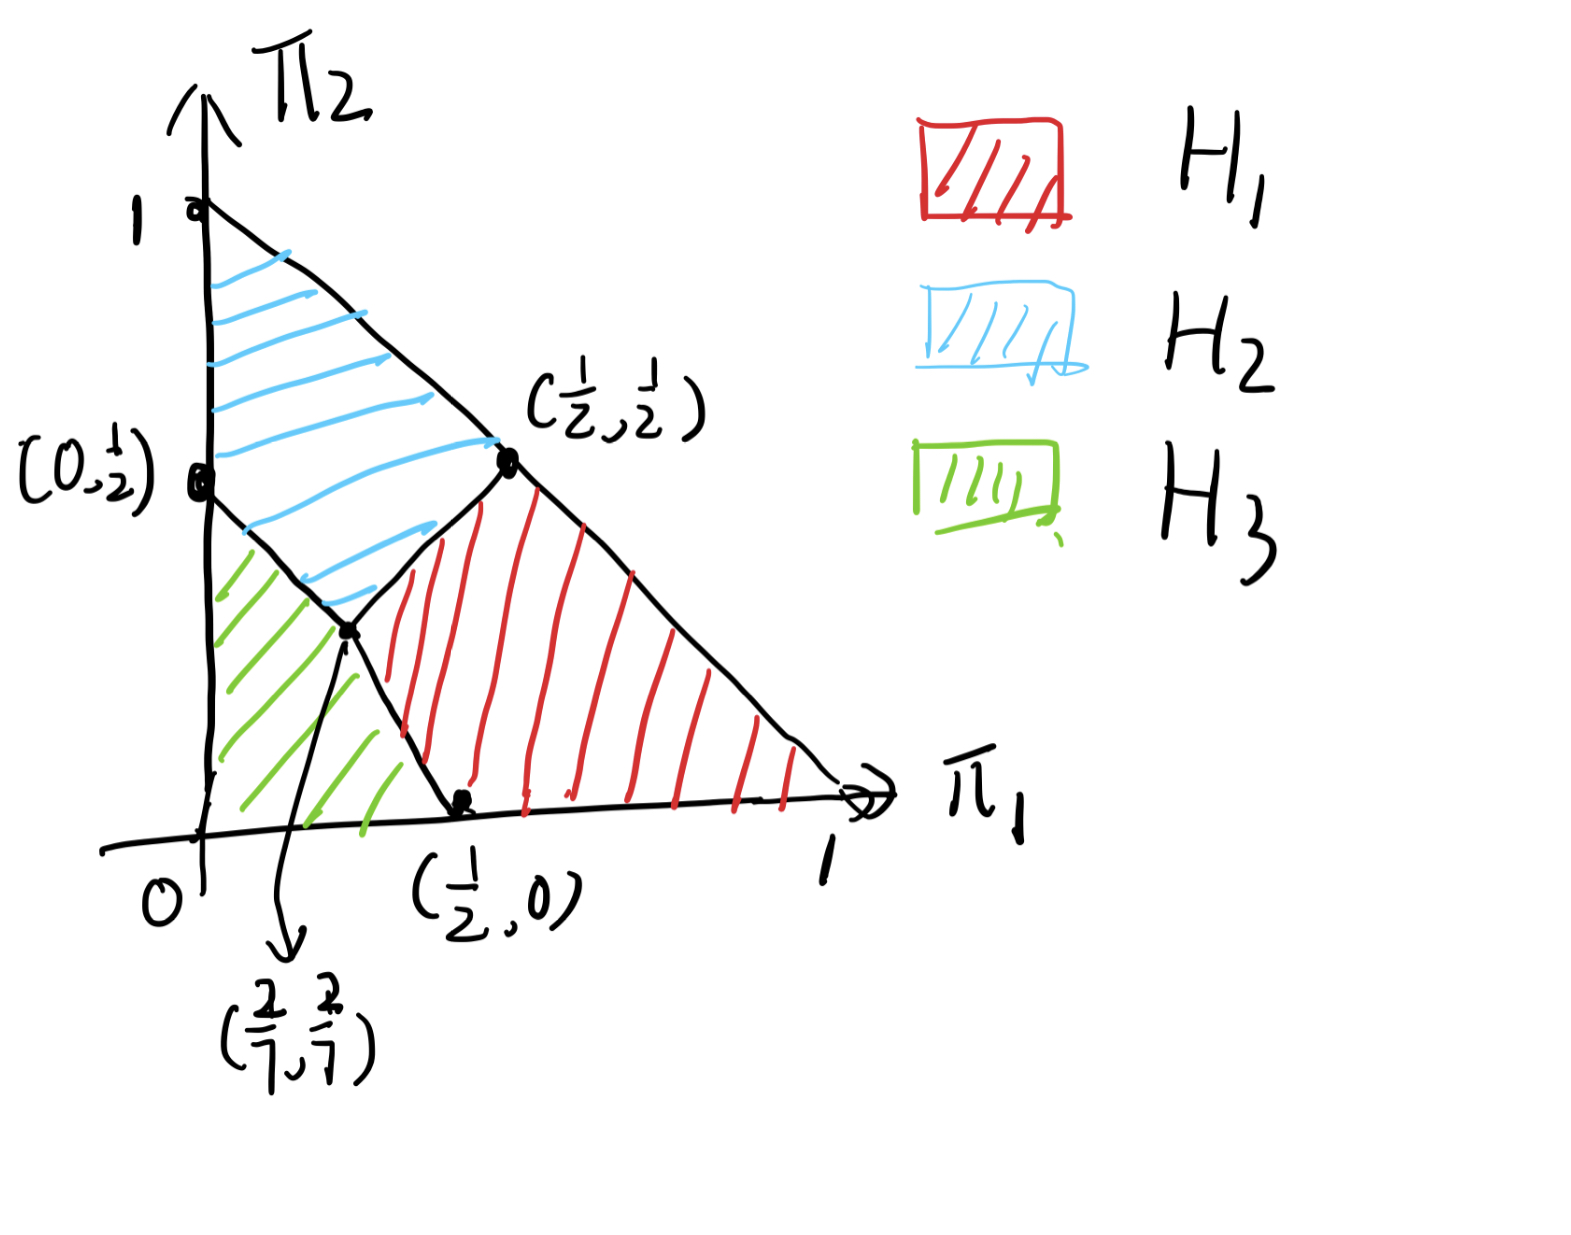
\includegraphics[width=0.5\linewidth]{decision-plane.png}
      \caption{Decision regions in the $(\pi_1, \pi_2)$ plane}
    \end{figure}
  \end{enumerate}

  \item When $C_{ij} = 1- \delta_{ij}$, the optimum decision rule is 
  
  \begin{equation}
    \hat H = f(\underline{y}) = \argmin_{i} \sum_{j=1}^3 C_{ij}\pi_i(\underline{y}) = \argmax_{i} \pi_i(\underline{y})
  \end{equation}

  Consider $L_{i}(\underline{y})=\frac{p_{\underline{\mathrm{y}} \mid \mathrm{H}}\left(\underline{y} \mid H_{i}\right)}{p_{\underline{\mathrm{y}} \mid \mathrm{H}}\left(\underline{y} \mid H_{1}\right)}$ for $i =2,3$, because three hypotheses are equally likely a priori, 

  \begin{equation}
    L_{i}(\underline{y})=\frac{p_{\underline{\mathrm{y}} \mid \mathrm{H}}\left(\underline{y} \mid H_{i}\right)}{p_{\underline{\mathrm{y}} \mid \mathrm{H}}\left(\underline{y} \mid H_{1}\right)} = \frac {\pi_i(\underline{y})} { \pi_1(\underline{y})}
  \end{equation}

  For consistency, denote $L_{1}(\underline{y})= 0$, so the optimum decision can be expresses in terms of $ L_{i}(\underline{y})$ as,

  \begin{equation}
    \hat H = \argmax_{i} \pi_i(\underline{y}) = \argmax_{i} L_i(\underline{y})
  \end{equation}

  To calculate $L_i(\underline{y})$,

  \begin{equation}
    L_i(\underline{y}) = \frac {\exp \left(-y_1^2 -(y_i-1)^2\right)}{\exp \left(-y_i^2 -(y_1-1)^2\right)} = \exp\left(2(y_i-y_1)\right),i=2,3
  \end{equation}

  So the optimum decision rule can be specfied in terms of the pair of suffcient statistics

  \begin{equation}
    \begin{array}{l}\ell_{2}(\underline{y})=y_{2}-y_{1} \\ \ell_{3}(\underline{y})=y_{3}-y_{1}\end{array}
  \end{equation}

  And the optimum decision rule is,

  \begin{equation}
    \hat H = f(\underline{y}) = \left\{
      \begin{aligned}
        &H_1,\ell_{2}(\underline{y})<0 \text{ and } \ell_{2}(\underline{y})<0 \\
        &H_2, \ell_{2}(\underline{y})>0 \text{ and } \ell_{2}(\underline{y})> \ell_{3}(\underline{y}) \\
        &H_3, \ell_{3}(\underline{y}) > 0 \text{ and }  \ell_{3}(\underline{y}) > \ell_{2}(\underline{y})
      \end{aligned}
      \right.
  \end{equation}
\end{enumerate}

\item \begin{enumerate}
  \item 
  At the local sensor,  $P(\mathrm{y_i} >0 | \mathrm{x}=1) = P(\mathrm{y_i} <0 | \mathrm{x}=-1)= 0.75$, 
  $P(\mathrm{y_i} <0 | \mathrm{x}=1)= P(\mathrm{y_i} >0 | \mathrm{x}=-1)= 0.25$.
  
  Thus, the conditional distribution of $\hat x_i$ given $\mathrm{x}$ is,

  \begin{equation}
    \begin{aligned}
      P(\hat x_i |\mathrm{x}=1 ) = 0.75^{\mathbf{I}(\hat x_i =1)} 0.25^{\mathbf{I}(\hat x_i =-1)} \\
      P(\hat x_i |\mathrm{x}=-1 ) = 0.75^{\mathbf{I}(\hat x_i =-1)} 0.25^{\mathbf{I}(\hat x_i =1)}
    \end{aligned}
  \end{equation}


At the fusion center, 

\begin{equation}
  \begin{aligned}
    P(\hat x_1, \hat x_2, \cdots, \hat x_n |\mathrm{x}=1 ) &= \prod_{i=1}^n  P(\hat x_i |\mathrm{x}=1 ) \\
    & = 0.75^{\sum_{i=1}^n \mathbf{I}(\hat x_i =1)} 0.25^{\sum_{i=1}^n \mathbf{I}(\hat x_i =-1)}\\
    P(\hat x_1, \hat x_2, \cdots, \hat x_n |\mathrm{x}=-1 ) &= \prod_{i=1}^n  P(\hat x_i |\mathrm{x}=-1 ) \\
    & = 0.75^{\sum_{i=1}^n \mathbf{I}(\hat x_i =-1)} 0.25^{\sum_{i=1}^n \mathbf{I}(\hat x_i =1)}
  \end{aligned}
\end{equation}

Denote $ m = \sum_{i=1}^n \mathbf{I}(\hat x_i =1)$ as the number of $1$-s in $\hat x_1, \hat x_2, \cdots, \hat x_n$, and because of equal probability priori,

\begin{equation}
  \begin{aligned}
    \frac{ P(\mathrm{x}=1 | \hat x_1, \hat x_2, \cdots, \hat x_n  )}{ P(\mathrm{x}=-1 | \hat x_1, \hat x_2, \cdots, \hat x_n  )} & = \frac{ P(\hat x_1, \hat x_2, \cdots, \hat x_n |\mathrm{x}=1 )}{ P(\hat x_1, \hat x_2, \cdots, \hat x_n |\mathrm{x}=-1 )}  \\
    & = 3^{2m-n}
  \end{aligned}
\end{equation}

So the minimum probability of error decision rule is a majority-voting rule as follows,


\begin{equation}
  \hat x (\hat x_1, \hat x_2, \cdots, \hat x_n) = \left\{
    \begin{aligned}
      1, \quad m \geqslant \frac  n 2 \\
      -1, \quad m < \frac n 2
    \end{aligned}
    \right.
\end{equation}

where $m$ denotes the number of one-s in $\hat x_1, \hat x_2, \cdots, \hat x_n$.


\item Suppose the local decision rule can be expressed as the conditional distriburion $p(\hat x_i | y_i)$of $\hat x_i$ given $y_i,i=1,2$. 

~\\

\textbf{Part 1}

First we prove that the decision rule is a deterministic rule, that is, given $y_i$, $\hat x_i$ is determined.

The expected joint cost is 

\begin{equation}
  \begin{aligned}
    \mathbb{E}\left[ C(\hat{x}_1,\hat x_2, x)\right] &= \sum_{\hat{x}_1,\hat x_2, x} C(\hat{x}_1,\hat x_2, x) p(\hat{x}_1,\hat x_2, x) \\
   & = \sum_{\hat{x}_1,\hat x_2, y_1,y_2,x} C(\hat{x}_1,\hat x_2, x) p(\hat{x}_1,\hat x_2, y_1,y_2,x) \\
   & = \sum_{\hat{x}_1,\hat x_2, y_1,y_2,x} C(\hat{x}_1,\hat x_2, x) p(\hat{x}_1 | y_1) p(\hat{x}_2 | y_2) p(y_1|x) p(y_2|x) p(x) \\
   & = \sum_{\hat x_2,y_1,y_2,x} \lambda(\hat x_2,y_1,y_2,x)[C(1,\hat{x}_2,x)p(\hat x_1 = 1|y_1) + C(-1,\hat{x}_2,x)p(\hat x_1 = -1|y_1)]\\
   & \quad \text{where } \lambda(\hat x_2,y_1,y_2,x) =  p(\hat{x}_2 | y_2) p(y_1|x) p(y_2|x) p(x) \\
   &\quad  (\text{Expanding the sum over } \hat x_1)
  \end{aligned}
\end{equation}

Assume $y_1$ is given, because  $p(\hat x_1 = -1|y_1) =1-p(\hat x_1 = 1|y_1)$, 

\begin{equation}
  \begin{aligned}
    \mathbb{E}\left[ C(\hat{x}_1,\hat x_2, x) | y_1  \right]  & = \sum_{\hat x_2,x} p_{\hat{\mathrm{x}}_2,\mathrm{x}}(\hat x_2,x) p_{\mathrm{y}_1 | \mathrm{x}}(y_1|x)\times \\ 
    & \quad \quad \left[\left(C(1,\hat{x}_2,x)-C(-1,\hat{x}_2,x)\right) p(\hat x_1 = 1|y_1) +C(-1,\hat{x}_2,x) \right]
  \end{aligned}
\end{equation}

To minimize $ \mathbb{E}\left[ C(\hat{x}_1,\hat x_2, x) | \hat x_2,y_1  \right]$, 

\begin{equation}
  p(\hat x_1 = 1|y_1) = \left\{ \begin{aligned}
    0, \quad \sum_{\hat x_2,x} p_{\hat{\mathrm{x}}_2,\mathrm{x}}(\hat x_2,x) p_{\mathrm{y}_1 | \mathrm{x}}(y_1|x)\left[C(1,\hat{x}_2,x)-C(-1,\hat{x}_2,x) \right] > 0 \\
    1, \quad\sum_{\hat x_2,x} p_{\hat{\mathrm{x}}_2,\mathrm{x}}(\hat x_2,x) p_{\mathrm{y}_1 | \mathrm{x}}(y_1|x)\left[C(1,\hat{x}_2,x)-C(-1,\hat{x}_2,x) \right] < 0
  \end{aligned}
  \right.
\end{equation}

which equals to,

\begin{equation}\label{eq:rule1}
    \hat x_1(y_1)= \left\{ \begin{aligned}
    1, \quad \sum_{\hat x_2,x} p_{\hat{\mathrm{x}}_2,\mathrm{x}}(\hat x_2,x) p_{\mathrm{y}_1 | \mathrm{x}}(y_1|x)\left[C(1,\hat{x}_2,x)-C(-1,\hat{x}_2,x) \right] < 0 \\
    -1, \quad \sum_{\hat x_2,x} p_{\hat{\mathrm{x}}_2,\mathrm{x}}(\hat x_2,x) p_{\mathrm{y}_1 | \mathrm{x}}(y_1|x)\left[C(1,\hat{x}_2,x)-C(-1,\hat{x}_2,x) \right] > 0
  \end{aligned}
  \right.
\end{equation}

~\\

\textbf{Part 2}

In this part we will prove the decision rule in Equation \ref{eq:rule1} can be seen as a form of a likelihood ratio test .

Expanding the sum over $x$,

\begin{equation}
  \begin{aligned}
    &\sum_{\hat x_2,x} p_{\hat{\mathrm{x}}_2,\mathrm{x}}(\hat x_2,x) p_{\mathrm{y}_1 | \mathrm{x}}(y_1|x)\left[C(1,\hat{x}_2,x)-C(-1,\hat{x}_2,x) \right] \\ = & \quad \sum_{\hat x_2} p_{\hat{\mathrm{x}}_2,\mathrm{x}}(\hat x_2,1) p_{\mathrm{y}_1 | \mathrm{x}}(y_1|1)\left[C(1,\hat{x}_2,1)-C(-1,\hat{x}_2,1) \right] \\ & \quad + \sum_{\hat x_2} p_{\hat{\mathrm{x}}_2,\mathrm{x}}(\hat x_2,-1) p_{\mathrm{y}_1 | \mathrm{x}}(y_1|-1)\left[C(1,\hat{x}_2,-1)-C(-1,\hat{x}_2,-1) \right]
  \end{aligned}
\end{equation}

Because the cost strictly increases with the number of errors made by the two sensors, so $C(1,\hat{x}_2,1)<C(-1,\hat{x}_2,1)$  and $C(1,\hat{x}_2,-1)>C(-1,\hat{x}_2,-1)$.

\begin{equation}
  \sum_{\hat x_2,x} p_{\hat{\mathrm{x}}_2,\mathrm{x}}(\hat x_2,x) p_{\mathrm{y}_1 | \mathrm{x}}(y_1|x)\left[C(1,\hat{x}_2,x)-C(-1,\hat{x}_2,x) \right]<0 \Longleftrightarrow \frac {p_{\mathrm{y}_1 | \mathrm{x}}(y_1|1)}{p_{\mathrm{y}_1 | \mathrm{x}}(y_1|-1)} > \gamma_1
\end{equation}

where $\gamma_1$ depends on the rule $\hat x_2(\cdot)$, 

\begin{equation}\label{eq:gamma}
  \gamma_1 = \frac {\sum_{\hat x_2} p_{\hat{\mathrm{x}}_2,\mathrm{x}} (\hat{x}_2,-1)\left[C(1,\hat{x}_2,-1)-C(-1,\hat{x}_2,-1) \right]}{ \sum_{\hat x_2} p_{\hat{\mathrm{x}}_2,\mathrm{x}} (\hat{x}_2,1)\left[C(-1,\hat{x}_2,1)-C(1,\hat{x}_2,1) \right]}
\end{equation}

And the decision rule for $\hat x_1(\cdot)$ is,

\begin{equation}
  \hat x_1(y_1)= \left\{ \begin{aligned}
  1, \quad \frac {p_{\mathrm{y}_1 | \mathrm{x}}(y_1|1)}{p_{\mathrm{y}_1 | \mathrm{x}}(y_1|-1)} > \gamma_1 \\
  -1, \quad \frac {p_{\mathrm{y}_1 | \mathrm{x}}(y_1|1)}{p_{\mathrm{y}_1 | \mathrm{x}}(y_1|-1)} < \gamma_1 
\end{aligned}
\right.
\end{equation}

\item In the same way,

\begin{equation}\label{eq:rule2}
  \hat x_2(y_2)= \left\{ \begin{aligned}
  1, \quad \frac {p_{\mathrm{y}_2 | \mathrm{x}}(y_2|1)}{p_{\mathrm{y}_2 | \mathrm{x}}(y_2|-1)} > \gamma_2 \\
  -1, \quad \frac {p_{\mathrm{y}_2 | \mathrm{x}}(y_2|1)}{p_{\mathrm{y}_2 | \mathrm{x}}(y_2|-1)} < \gamma_2
\end{aligned}
\right.
\end{equation}

where 

\begin{equation}
  \gamma_2 = \frac {\sum_{\hat x_1} p_{\hat{\mathrm{x}}_1,\mathrm{x}} (\hat{x}_1,-1)\left[C(\hat{x}_1,1,-1)-C(\hat{x}_1,-1,-1) \right]}{ \sum_{\hat x_1} p_{\hat{\mathrm{x}}_1,\mathrm{x}} (\hat{x}_1,1)\left[C(\hat{x}_1,-1,1)-C(\hat{x}_1,1,1) \right]}
\end{equation}

\item As the Equation \ref{eq:gamma} shows, 

\begin{equation}\label{eq:gamma}
  \begin{aligned}
    \gamma_1 & = \frac { p_{\hat{\mathrm{x}}_2,\mathrm{x}} (1,-1)\left[C(1,1,-1)-C(-1,1,-1) \right] + p_{\hat{\mathrm{x}}_2,\mathrm{x}} (-1,-1)\left[C(1,-1,-1)-C(-1,-1,-1) \right]}{  p_{\hat{\mathrm{x}}_2,\mathrm{x}} (1,1)\left[C(-1,1,1)-C(1,1,1) \right]+ p_{\hat{\mathrm{x}}_2,\mathrm{x}} (-1,1)\left[C(-1,-1,1)-C(1,-1,1) \right]}  \\
    & = \frac { p_{\hat{\mathrm{x}}_2,\mathrm{x}} (1,-1)(L-1) + p_{\hat{\mathrm{x}}_2,\mathrm{x}} (-1,-1)}{  p_{\hat{\mathrm{x}}_2,\mathrm{x}}(1,1) + p_{\hat{\mathrm{x}}_2,\mathrm{x}} (-1,1)(L-1)}
  \end{aligned}
\end{equation}

Because $ p_{\hat{\mathrm{x}}_2,\mathrm{x}} (1,-1) +p_{\hat{\mathrm{x}}_2,\mathrm{x}} (-1,-1)  = p_{\mathrm{x}}(x=-1)$ and $ p_{\hat{\mathrm{x}}_2,\mathrm{x}} (1,1) +p_{\hat{\mathrm{x}}_2,\mathrm{x}} (-1,1)  = p_{\mathrm{x}}(x=1)$,

\begin{equation}\label{eq:gamma}
  \begin{aligned}
    \gamma_1  & = \frac { (L-2)p_{\hat{\mathrm{x}}_2,\mathrm{x}} (1,-1) + p_{\mathrm{x}}(x=-1)}{ (L-2) p_{\hat{\mathrm{x}}_2,\mathrm{x}}(-1,1) +p_{\mathrm{x}}(x=1)}
  \end{aligned}
\end{equation}


So when $L=2,\gamma_1 = \frac {p_{\mathrm{x}}(x=-1)}{p_{\mathrm{x}}(x=1)}$ does not depend on $\hat x_2(\cdot)$.

\item \textbf{Some thoughts}: 

It is also interesting when $L\neq 2$.

\begin{itemize}
  \item When $1<L<2$, double errors are discounted relatively comparing to single error, which encourages local decisions to be more bold.
  \item When $L>2$, double errors become more expensive. As $L$ increases, to avoid double errors, $\hat x_1$ and $\hat x_2$ even may be always opposite!
\end{itemize}

\end{enumerate}



\end{enumerate}
\end{document}
%%% Local Variables:
%%% mode: latex
%%% TeX-master: t
%%% End:
